\documentclass[a4paper]{article}

\usepackage[utf8]{inputenc}
\usepackage[T1]{fontenc}
\usepackage{textcomp}
\usepackage[english]{babel}
\usepackage{amsmath, amssymb, amsthm}
\usepackage{tikz}
\usepackage{pgfplots}
\usetikzlibrary{calc, arrows.meta, positioning, angles, quotes, patterns}



% figure support
\usepackage{import}
\usepackage{xifthen}
\pdfminorversion=7
\usepackage{pdfpages}
\usepackage{transparent}
\usepackage{hyperref}
\usepackage[margin=0.8in]{geometry}
\usepackage{float}

\usepackage{setspace}
% \setlength{\parindent}{0in}

\pdfsuppresswarningpagegroup=1

\newcommand{\N}{\mathbb{N}}
\newcommand{\R}{\mathbb{R}}
\newcommand{\Z}{\mathbb{Z}}
\newcommand{\Q}{\mathbb{Q}}

\newtheorem{theoreme}{Théorème}[section]
\newtheorem{definition}{Définition}[section]
\newtheorem{exemple}{Exemple}[section]
\newtheorem{proposition}{Proposition}[section]
\newtheorem{propriete}{Propriété(s)}[section]
\newtheorem*{notation}{Notation}
\newtheorem*{remarque}{Remarque}

\author{Yehor Korotenko}
\title{Oraux de Maths: Séance 1}
\newcommand{\scalair}[1]{\langle #1 \rangle}

\newcommand{\incfig}[1]{%
    \def\svgwidth{\columnwidth}
    \import{./figures/}{#1.pdf_tex}
}

\begin{document}
   \maketitle 
   \section{Algèbre Linéaire}
   En algèbre linéaire on a toujours besoin de calculer les coordonnées d'un vecteur dans une bases. Habituelement, cela prend pas mal de temps pour résoudre un système linéaire. 
   Heureusement, dans $\R^n$ il existe une façon plus facile et plus vite de trouver tels coordonnées: base orthonormé. 
    \par
        Soit un vecteur  $x \in E := \R^2$ et  $v_1, v_2 \in \R^2$ une base quelconque, $e_1, e_2 \in \R^2$ base orthonormée. Alors:
        \begin{align*}
            \exists a_1, a_2 \in \R \quad &x = a_1v_1 + a_2v_2\\
            \text{et }                    &x = \scalair{x, e_1}e_1 + \scalair{x, e_2}e_2 \quad \text{ (d'après le cours)}
        \end{align*}
\begin{figure}[H]
    \centering
    \incfig{fig-1}
    \caption{fig-1}
    \label{fig:fig-1}
\end{figure}
Pourquoi ne peut-on pas calculer les coordonnées de même façon dans une base usuelle?: (draw grid)
\begin{align*}
    \scalair{x, e_1} &= \scalair{\scalair{x, e_1}e_1 + \scalair{x, e_2}e_2, e_1}\\
                     &= \scalair{x, e_1}\underbrace{ \scalair{e_1,e_1} }_{= 1} + \scalair{x, e_2}\underbrace{\scalair{e_2, e_1}}_{= 0}\\
                     &= \scalair{x, e_1}\\
    \scalair{x, v_1} &= \scalair{a_1v_1 + a_2v_2, v_1}\\
                     &= a_1\scalair{v_1, v_1} + a_2\underbrace{ \scalair{v_2, v_1} }_{\substack{\text{une contribution de $v_2k$}\\\text{dans le produit $\scalair{x, v_1}$}}}
\end{align*}
Donc le produit $\scalair{x, v_1}$ ne donne pas les vrai coordonnées par rapport à $v_1$.
\par
Bonne nouvelle: dans $\R^n$ il existe toujours une base orthonormée.
\begin{theoreme}\label{thm:thm-fond}
   fondamentale d'Algèbre Linéaire. \par
   (Expliquer remarque, que orthogonaux donne orthonormal et que deux à deux arthogonaux $\implies$ libre)\par
   Dans un éspace euclidien il existe toujours des bases orthonormées.
\end{theoreme}
\begin{proof} de {Théorème \ref{thm:thm-fond}}\par
   Il suffit de montrer qu'il existe des bases orthogonales car on peut les toujours normé. Alors, montrons par récurrence sur la dimension $n$ de  $E$. Pour  $n = 1$ il n'y a rien à demontrer car on a seulement un vecteur dans une base. Supposons que le théorème est vrai à l'ordre  $n - 1$ et soit  $v \in E, \, v \neq 0$. Considérons l'ensemble de tous les vecteurs orthogonaux à $v$:
   \[
       F = \{x \in E \mid \scalair{x, v} = 0\}
   \] 
   On voit bien que $dim(F) = n - 1$. En effet, soit  une application $\omega(x) = \scalair{x, v}$. On voit bien que  $F = Ker(\omega)$ et  $dim(Im(\omega)) = 1$ alors par le théorème du rang on obtient que  
   \[
       dim(Ker(\omega)) = \underbrace{dim(E)}_{= n} - \underbrace{dim(Im(\omega))}_{= 1} = n - 1
   \] 
   car $\omega(v) = \|v\| \neq 0$ et $\omega \neq 0$. Donc, par l'hypothèse de récurrence, il existe des bases orthogonales de $F$ pour dimension  $n - 1$. De plus,  $v \not\in F$, car si on avait  $v \in F$ on aurait  $\scalair{v, v} = 0 \implies v = 0$ ce qui contredit avec l'hypothese. Aussi, $E = Vect\{v\} \oplus F$. Par conséquent, il existe une base orthogonale $\{v_2, \ldots, v_n\}$ pour $F$ et  $v$ est orthogonale  à chaque vecteur de base de $F$, d'où  $\{v_1, \ldots, v_n\}$ est une base orthogonale de $E$. Ce qu'il fallait démontrer. 
\end{proof}
\begin{theoreme}\label{thm:gram-schmidt}
   de Gram-Schmidt.\par 
   Soit $(E, \scalair{,})$ un éspace euclidien. Soit  $F$ sous-espace de  $E$ engendré par une famille  $\{v_1, \ldots, v_n\}$. Alors, il existe une famille orthogonale $\{w_1, \ldots, w_p\}$ tel que $Vect\{v_1, \ldots, v_p\} = Vect\{w_1, \ldots, w_p\}$.
   \par Remarque: ce théorème nous donne aussi un procédé d'orthonormalisation.
\end{theoreme}
\begin{proof} du Théorème \ref{thm:gram-schmidt}
    Construisons la base orthogonale: $\{w_1, \ldots, w_p\}$. Posons d'abord:
    \[
    \begin{cases}
        w_1 = v_1\\
        w_2 = v_2 + \lambda w_1, \qquad \text{avec } \lambda \text{ tel que } w_1 \perp w_2
    \end{cases}
    \] 
    En imposant cette condition on trouve:
    \[
        0 = \scalair{v_2 + \lambda w_1, w_1} = \scalair{v_2, w_1} + \lambda \|w_1\|^2
    \] 
    Comme $w_1 \neq 0$, on obtient $\lambda = - \frac{\scalair{v_2, w_1}}{\|w_1\|^2}$. On remarque que:
    \[
    \begin{cases}
        v_1 = w_1\\
        v_2 = w_2 - \lambda w_1
    \end{cases}
    \] 
    donc $Vect\{v_1, v_2\} = Vect\{w_1, w_2\}$.
    \par
    On peut voir $w_2 = v_2 - \lambda' w_1 $ comme $w_2 = v_2 - proj_{F_1}v_2$ où $F_i = Vect\{w_1, \ldots, w_i\}$
    \begin{figure}[ht]
        \centering
        \incfig{projection-with-bon}
        \caption{Projection avec BON}
        \label{fig:projection-with-bon}
    \end{figure}
    \par
    Mais, c'est quoi une projection?
\begin{figure}[H]
   \centering 
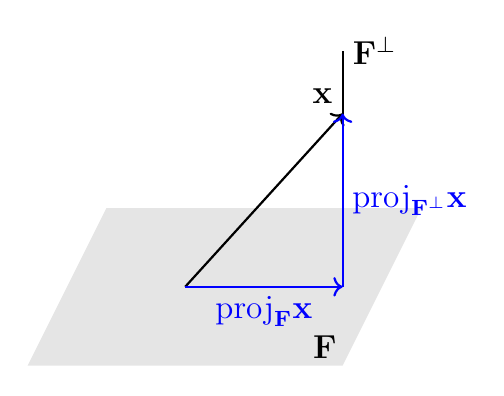
\begin{tikzpicture}

% Draw the plane
\fill[gray!20] (-2,-1) -- (2,-1) -- (3,1) -- (-1,1) -- cycle;

% Draw the vectors
\draw[->, thick, black] (0,0) -- (2,2.2) node[anchor=south east] {\large $\mathbf{x}$};

\node[anchor=north, blue] (_) at ($(0,0)!0.5!(2,0)$) {\large $\text{proj}_\mathbf{F} \mathbf{x}$};
\node[anchor=west, blue] (_) at ($(2,0)!0.5!(2,2.2)$) {\large $\text{proj}_\mathbf{F^{\perp}} \mathbf{x}$};
% Add the labels for w and w perpendicular
\draw[->, thick, blue] (0,0) -- (2,0) ;
\draw[thick, black] (2,0) -- (2,3) node[anchor=west] {\large $\mathbf{F}^\perp$};
\draw[->, thick, blue] (2,0) -- (2,2.2);
\node[anchor=north west] (_) at (1.5, -0.5) {\large $\mathbf{F}$};
% Add the right angle symbol

\end{tikzpicture}
\caption{Projection}
\label{pic:projection}
\end{figure}

    \par
    Une fois construit $w_2$, on construit $w_3$ en posant:
    \begin{align*}
        &w_3 = v_3 + \mu w_1 + \nu w_2\\
        &\text{avec } \mu \text{ et } \nu \text{ tels que: } w_3 \perp w_1 \text{ et } w_3 \perp w_2
    \end{align*}
    Ceci donne
    \begin{align*}
        0 &= \scalair{v_3 + \mu w_1 + \nu w_2, w_1} = \scalair{v_3, w_1} + \mu \underset{= \|w_1\|^2}{\scalair{w_1, w_1}} + \nu \underset{= 0}{\scalair{w_2, w_1}}\\
          &= \scalair{v_3, w_1} + \mu \|w_1\|^2 
    \end{align*}
    d'où $\mu = - \frac{\scalair{v_3, w_1}}{\|w_1\|^2}$. De même, en imposant que $w_3 \perp w_2$, on trouve $\nu = - \frac{\scalair{v_3, w_2}}{\|w_2\|^2}$. Comme
    \[
    \begin{cases}
        v_1 = w_1\\
        v_2 = w_2 - \lambda w_1\\
        v_3 = w_3 - \mu w_1 - \nu w_2
    \end{cases}
    \] 
    on voit bien que $Vect\{w_1, w_2, w_3\} = Vect\{v_1, v_2, v_3\}$. C'est-à-dire, $\{w_1, w_2, w_3\}$ est une base orthogonale de l'éspace engendre par $v_1, v_2, v_3$. On voit bien maintenant le procédé de récurrence.
    \par
    Supposons avoir construit $w_1, \ldots, w_{k-1}$ pour $k \le p$. On pose:
    \begin{align*}
        w_k &= v_k + \text{ combinaison linéaire des vecteurs déjà trouvés}\\
            &= v_k + \lambda_1w_1 + \ldots + \lambda_{k-1}w_{k-1}
    \end{align*}
    Les conditions $w_k \perp w_i$ (pour $i \in \{1, \ldots, k-1\}$) sont équivalentes à:
    \[
        \lambda_i = - \frac{\scalair{v_k, w_i}}{\|w_i\|^2}
    \] 
    comme on le vérifie immédiatement. Puisque $v_k = w_k - \lambda_1 - \ldots - \lambda_{k-1}w_{k-1}$, on voit par récurrence que $Vect\{w_1, \ldots, w_k\} = Vect\{v_1, \ldots, v_k\}$ $\iff$ $\{w_1, \ldots, w_k\}$ eset une base orthogonale de $Vect\{v_1, \ldots, v_k\}$.
    \par
    Ce qu'il nous rester c'est à la normaliser, i.e  $\forall i \in \{1, \ldots, k\}$ $e_i = \frac{w_i}{\|w_i\|}$, d'où $\{e_1, \ldots, e_k\}$ est une base orthonormale de $F = Vect\{v_1, \ldots, v_k\}$.
\end{proof}
\end{document}
